% Autogenerated translation of about.md by Texpad
% To stop this file being overwritten during the typeset process, please move or remove this header

\documentclass[12pt]{book}
\usepackage{graphicx}
\usepackage{fontspec}
\usepackage[utf8]{inputenc}
\usepackage[a4paper,left=.5in,right=.5in,top=.3in,bottom=0.3in]{geometry}
\setlength\parindent{0pt}
\setlength{\parskip}{\baselineskip}
\setmainfont{Helvetica Neue}
\usepackage{hyperref}
\pagestyle{plain}
\begin{document}

\hrule
permalink: /
title: ""
excerpt: "About me"
author\emph{profile: true
redirect}from: 
  - /about/

\section*{  - /about.html}

\begin{itemize}
\item I am a Ph.D. candidate in Statistics at King Abdullah University of Science and Technology (KAUST) with Prof. \href{https://cemse.kaust.edu.sa/stat/people/person/raphael-huser}{Raphaël Huser}. I obtained my bachelor's degree in financial mathematics at Southern University of Science and Technology (SUSTech), Shenzhen, China, in 2017 and a master's degree in Statistics at KAUST in 2018. My research mainly focuses on modeling spatial extremes, high-dimensional inference, and Bayesian inference. In addition, I am also interested in deep learning frameworks, e.g., GAN and VAE (Variational Autoencoder). 
\item \textbf{I am now in the job market and am looking for a postdoc position in related fields}.  
\item Here is a photo of 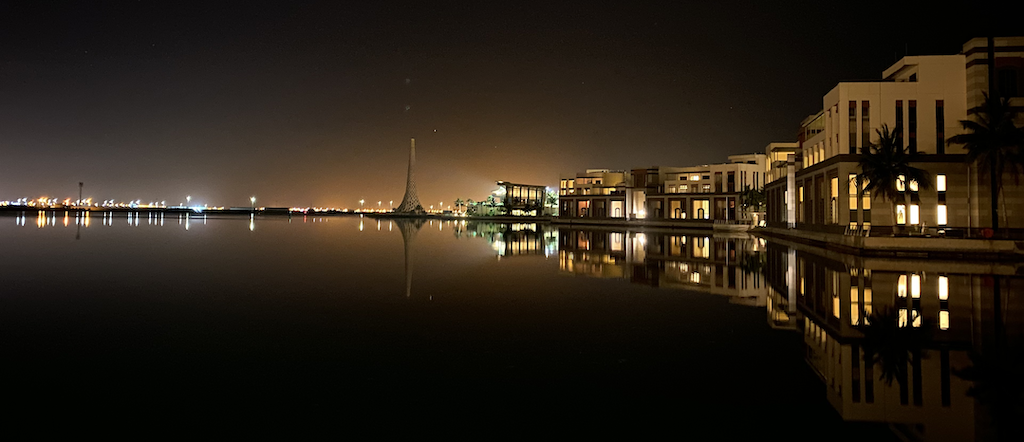
\includegraphics{../images/KAUST.png}
\end{itemize}

\chapter*{Publications}

\begin{itemize}
\item \textbf{Peng Zhong}, \href{https://cemse.kaust.edu.sa/stat/people/person/raphael-huser}{Raphaël Huser}, and \href{https://biosp.mathnum.inrae.fr/homepage-thomas-opitz}{Thomas Opitz}, \textbf{Exact simulation of max-infinitely divisible processes}, \emph{Econometrics and Statistics, accepted, 2022+} \href{files/paper2.pdf}{link} 
\item \textbf{Peng Zhong}, \href{https://cemse.kaust.edu.sa/stat/people/person/raphael-huser}{Raphaël Huser}, and \href{https://biosp.mathnum.inrae.fr/homepage-thomas-opitz}{Thomas Opitz}, \textbf{Modeling non-stationary temperature maxima based on extremal dependence changing with event magnitude}, \emph{Annals of Applied Statistics, to appear, 2022} \href{files/paper1.pdf}{link}
\end{itemize}

\end{document}
